\chapter{\emph{gem}- and \emph{vic} Disubstitutions}%
\label{ch:gem-vic-disubstitions}

The source of kinetic effect in the geminal substitution is similar to the one
commonly involved in enzyme catalysis:
the intramolecular reaction rate can be
increased by rearranging the substrate reactive centers in a way similar to the
steric configuration corresponding to the transition state, which is itself a
consequence of the Bells-Evans-Polanyi (BEP) principle.

This steric compression can be obtained by the introduction of geminal
disubstitutions (\emph{gem}-) in the chain conecting two reaction centers
(\cref{fig:gem-dimetila}):
when \emph{cis} reacting groups are held close in a rigid system,
those reactions take place faster than
otherwise~\cite{Beesley_1915,Allinger_1960,Bruice_1960a,Bruice_1960b,Capon_1964,Bruice_1965,Kirby_1972,Galli_1979,Kirby_1980,Lightstone_1994,Kaneti_2004,Jung_2005,Karaman_2011}.
%
\begin{figure}[hbtp]
	\centering
	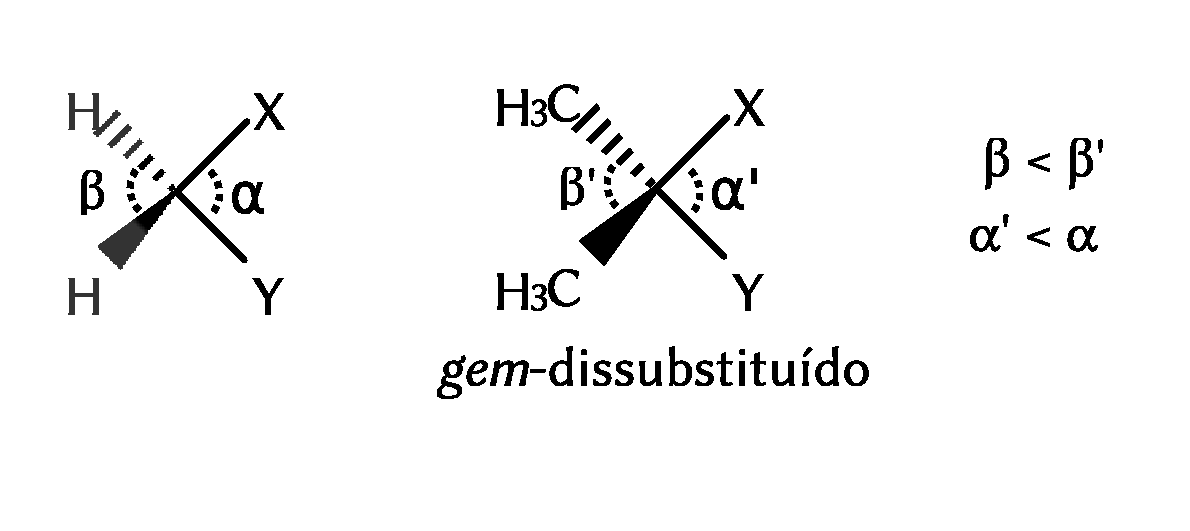
\includegraphics[width=.55\textwidth]{figures/gem-dimetil-pt}
	\caption[Beesley-Thorpe-Ingold effect, also known as geminal dimethyl
		effect.]{
		\emph{gem}-Dimethyl substitution (center), a kind of
		\emph{gem}-disubstitution.
		According to Beesley, Thorpe and Ingold~\cite{Beesley_1915,Jung_2005},
		such substitutions promote the increase of the $\beta$ angle and the
		decrase of the $\alpha$ angle (so called ``Beesley-Thorpe-Ingold''
		effect, or ``geminal dimethyl effect''),
		when compared to the non-substituted structure (left),
		which brings the reactive centers
		\ce{X} and \ce{Y}
		closer together.
		The reactive centers \ce{X} and \ce{Y} can consist of
		carbonic chains,
		which allow the formation of rings of arbitrary size.}\label{fig:gem-dimetila}
\end{figure}
%
The alkyl \emph{gem}-disubstitution effect,
already known and studied for more than a century,
is the name given to the increase in cyclization rate due
to the substitution of hydrogen atoms by alkyl groups in carbons in the
tethering chain that connects two reactive centers (\ce{X} and \ce{Y}
in~\cref{fig:gem-dimetila}, for example)~\cite{Capon_1964,Kirby_1980,Kaneti_2004,Jung_2005}.

The present of vicinial alkyl groups in the chain undergoing cyclyzation
indices a similar kinetic effect (\emph{vic}-disubstitution)
to the \emph{gem}-dialkyl one.
One example that allows a comparison between the two
involves the anhydride formation from monoesters of many diacid
succinates~\cite{Kirby_1980,Bruice_1960a,Bruice_1960b,Bruice_1965,Lightstone_1994}
(\cref{fig:succinatos}), whose relative reaction rates
$k_\text{rel}$ span one order of magnitude.
%
\begin{figure}[hbtp]
	\centering
	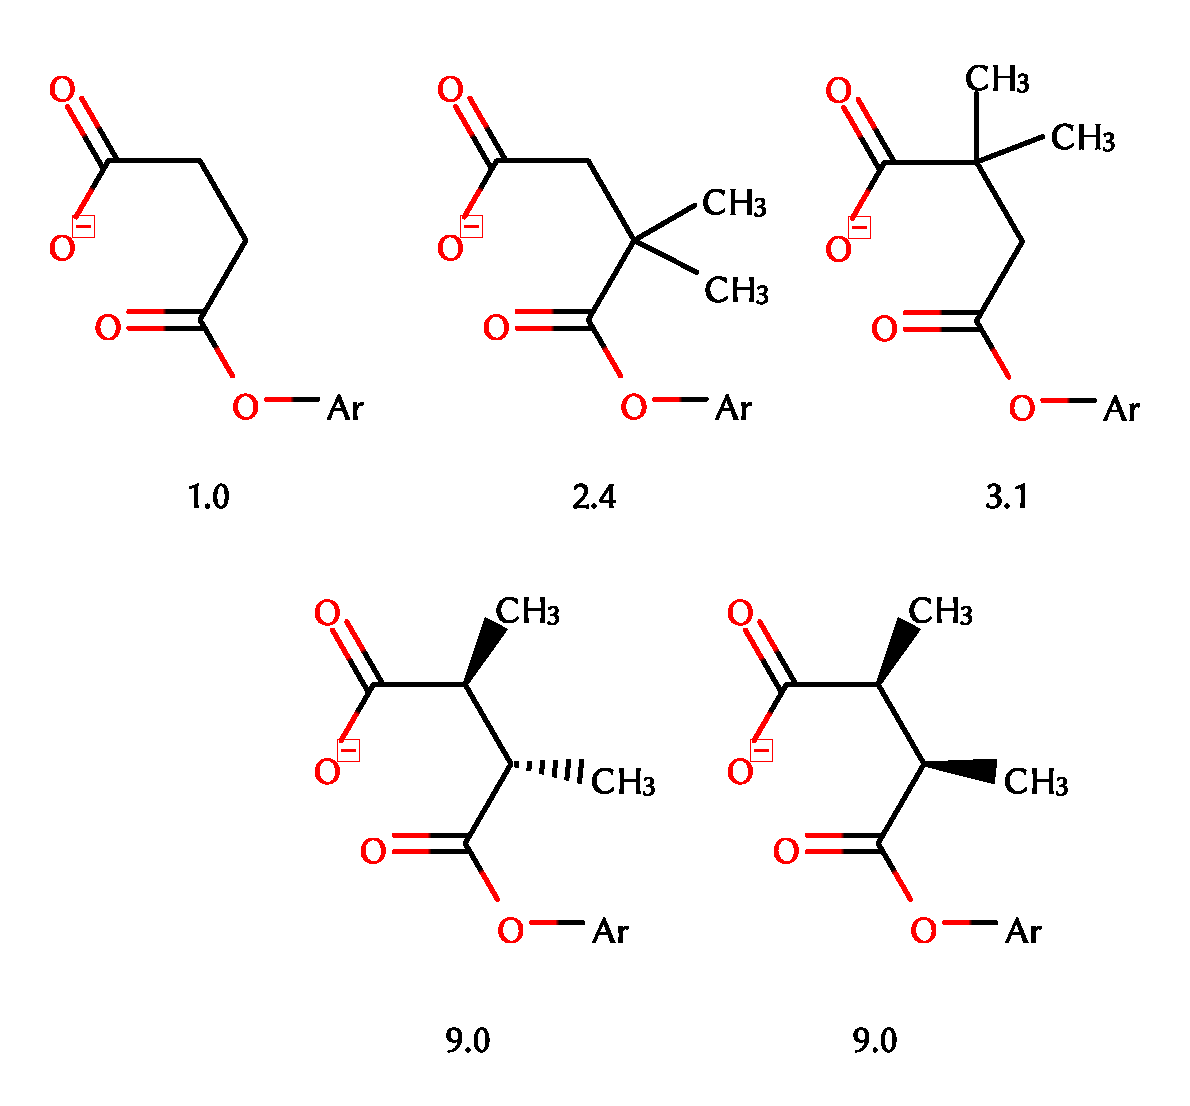
\includegraphics[width=.75\textwidth]{figures/succinatos}
	\caption[Kinetic effects of geminal and vicinal disubstitutions.]{
		Kinetic effect of geminal disubstitution when compared to the vicinal disubstitution.
		The relative cyclization rate ($k_\text{rel}$)
		is shown under each compound.}\label{fig:succinatos}
\end{figure}
%
In this case, the
cyclization rate
of the
\emph{vic}-dimethyl substituted
succinate
is significantly higher than the \emph{gem}-dimethyl substituted one
(\cref{fig:succinatos}).

Another staggering example of the vicinal effect is found in
\ce{N}-alkyl substituted maleamic acids~\cite{Kirby_1972,Karaman_2011} (\cref{fig:acidos_maleamicos}),
whose structures are more rigid than the ones of the
succinates mentioned above.
In fact, the substituent effect in this class of reactions span ten
orders of magnitude in
$k_\text{rel}$ ($10^{-6}$--$10^{4}$,~\cref{fig:acidos_maleamicos}).
%
\begin{figure}[hbtp]
	\centering
	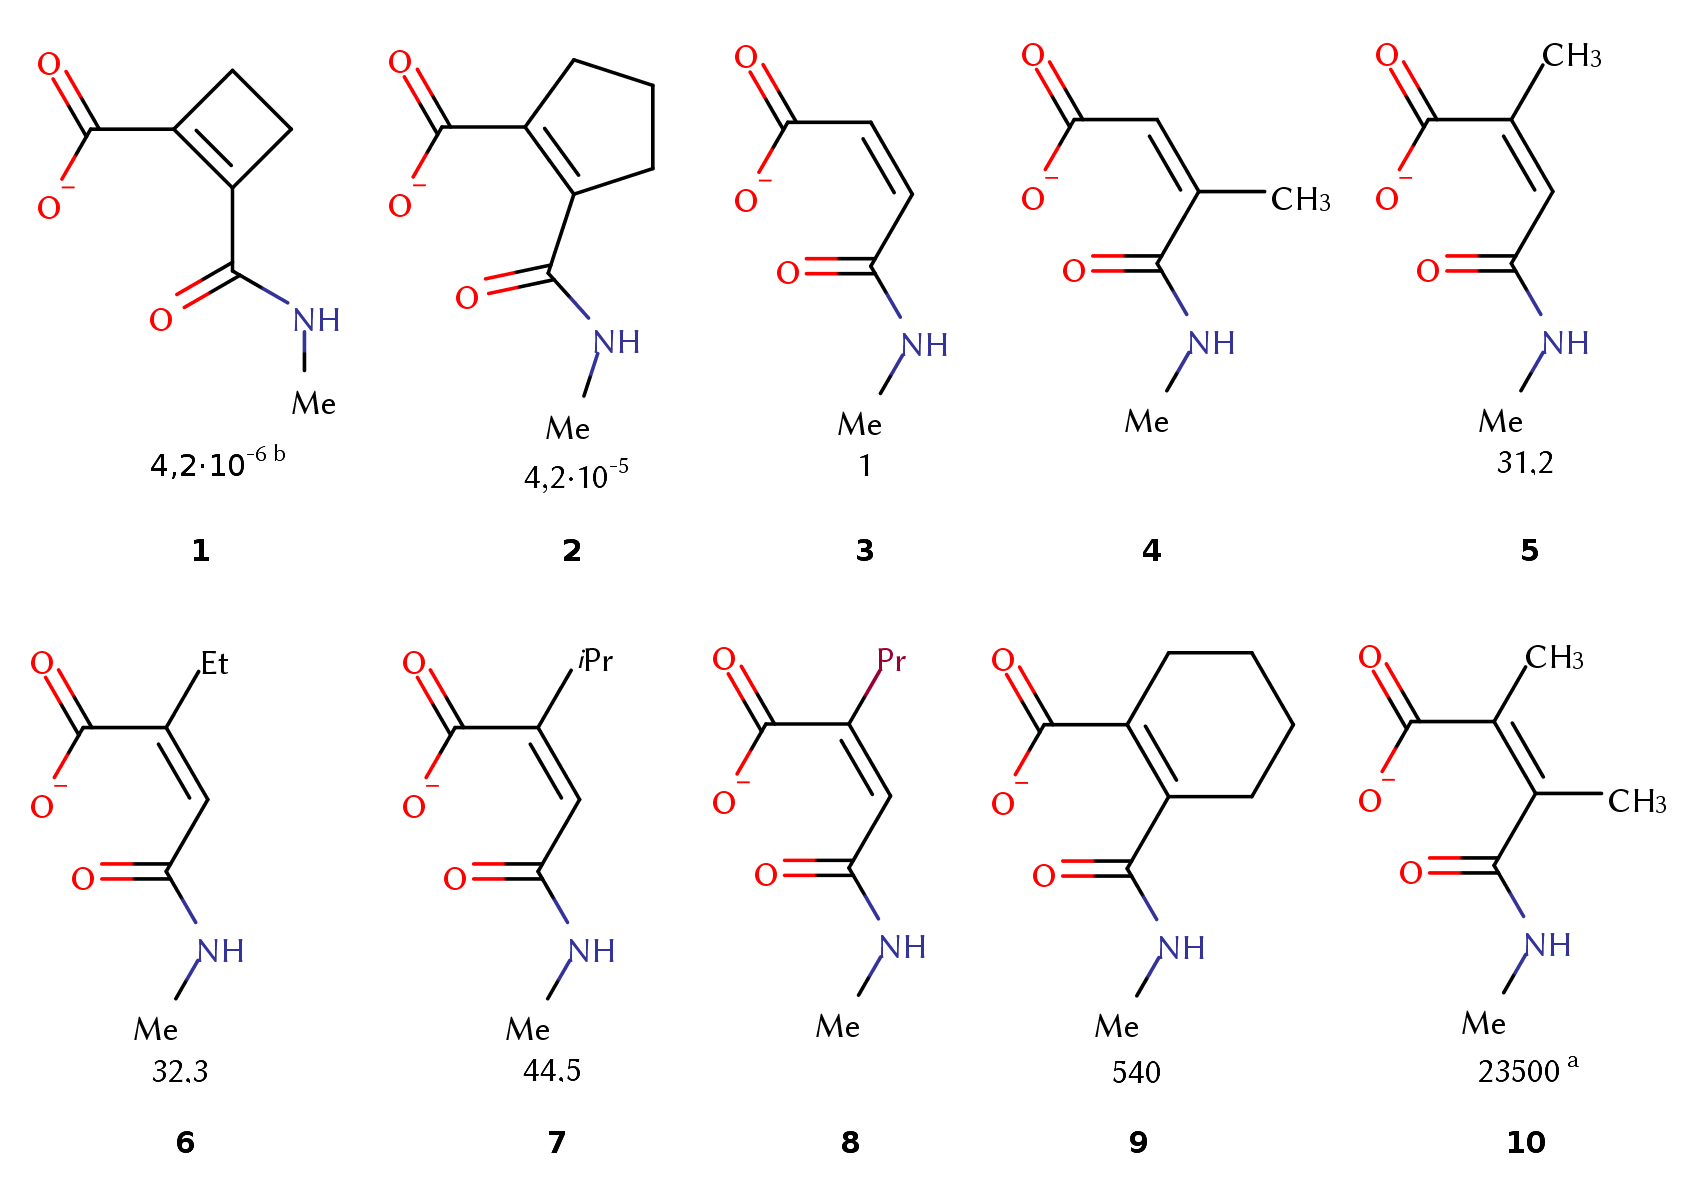
\includegraphics[width=.8\textwidth]{figures/acidos_maleamicos}

	\textbf{(a)}

	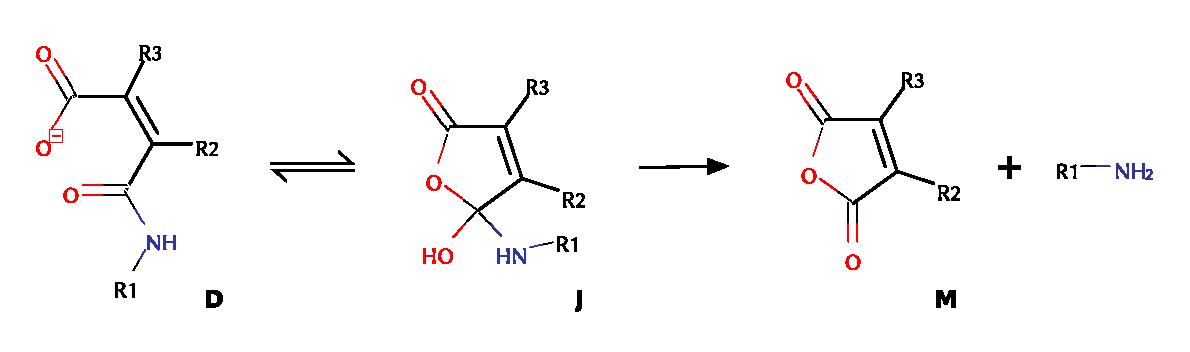
\includegraphics[width=.8\textwidth]{figures/acidos_maleamicos_reacao}

	\textbf{(b)}

	\caption[Intramolecular hydrolysis of the amidic bond in maleamic acids and
		their \ce{N}-methyl substitutional kinetic effect.]{
		\textbf{(a)}
		Substitutional kinetic effect in \ce{N}-methyl
		maleamic acids for the cyclization reaction shown in \textbf{(b)}.
		Such structure only admit vicinal disubstitutions.
		Available reaction rate constants $k_\text{rel}$ available in
		the literature (relative to compound \textbf{3}, measured at 39°C)
		are shown under each compound~\cite{Kirby_1972}.
		$^a$Originally estimated from a similar structure~\cite{Kirby_1972}.
		$^b$Estimated from 100°C measurements due to slow reaction rate~\cite{Kirby_1972}.
		\textbf{(b)}
		Intramolecular hydrolysis of the amidic bond of \ce{N}-alkyl
		substituted maleamic acids, giving rise to the formation of maleamic
		anhydride derivatives~\cite{Kirby_1972,Jung_2005,Karaman_2011}.}%
	\label{fig:acidos_maleamicos}
\end{figure}
%
Such structures undergo cyclization and intramolecular hydrolysis of the amidic
bond, resulting in the formation of maleamic anhydride derivatives (\cref{fig:acidos_maleamicos}).
The breakdown of the amidic bond allows us to classify the reaction as mimetic
to the one catalytic promoted by peptidases~\cite{Kirby_1972},
which are of great importance in many biological processes such as
digestion~\cite{Lehninger_2012}, programmed cell death~\cite{Fesik_2001},
cancer cell development~\cite{Kenny_1989},
the widespread of crop diseases~\cite{Kapust_2000},
and biochemical signaling in living
organisms~\cite{Lehninger_2012,Borissoff_2009}.
Being more rigid, it is expected that those componds present higher reaction
rates, as evidenced by fact that substrates closer to the active site of
enzymes is enough for the enzymatic behavior~\cite{Souza_2017},
although such view in general has been questioned by other authors~\cite{Nobel_2013};
it is not reasonable, on the other hand, to believe that the distance between
reactive centers is not a key factor in catalysis.
